% :encoding=UTF-8:
% -*- TeX:FR -*-
\documentclass[12pt,oneside]{paper}
\usepackage{authblk}
\usepackage[datesep={},hourminsep={},useregional]{datetime2}

\usepackage[
	xetex,
	bookmarks=true,bookmarksopen,
	colorlinks=true,citecolor=blue,urlcolor=BleuTor,linkcolor=black,
	pdfauthor={Vincent BAIN},
	pdftitle={Manuel r.avac},
	pdfsubject={Code avalanches coulantes AVAC : utilisation avec GRASS GIS}]{hyperref}
	

\hypersetup{
pdfinfo={
CreationDate={D:201910221700},
ModDate={D:\DTMnow}
}
}
\usepackage[
	a4paper,
	vscale=1,
	top=2.5cm,
	bottom=2.5cm,
	left=2.5cm,
	right=2.5cm]{geometry}
\usepackage[T1]{fontenc}
\usepackage{amsmath,bm}
\usepackage{french}
\usepackage{color}
\usepackage[xetex]{graphicx}
\usepackage{fancyhdr}
\usepackage{titlesec}
\usepackage{fancyvrb}
\usepackage{manfnt}

\definecolor{gris.3}{gray}{0.3}
\definecolor{gris.5}{gray}{0.5}
\definecolor{noir}{gray}{0}
\definecolor{BleuTor}{rgb}{0,0.53,0.72}

\titleformat*{\subsection}{\bfseries}
\titleformat*{\paragraph}{\bfseries}

\newcommand{\esp}{\vskip0.3cm}
\newcommand{\comment}[1]{\marginpar{\begin{flushleft}  #1\end{flushleft}}}

\newenvironment{code}{%
\vspace{2mm}%
\hangindent=.6cm%
\parindent.6cm%
\ttfamily%
\color{gris.3}%
}{
\vspace{2mm}%
}

\makeatletter
\addto\captionsfrench{\renewcommand{\fnum@figure}{\small\textbf{\figurename~\thefigure~}}}
\makeatother

\addto\captionsfrench{\def\figurename{{\small Figure}}}
\addto\captionsfrench{\def\CaptionSeparator{. \space}}
\def\captionseparator{. \space}
\addto\captionsfrench{\def\captionfont{\small}}

\setlength{\parskip}{5pt}

%fontes
%..............................
\usepackage{fontspec}
\defaultfontfeatures{Mapping=tex-text}
\setmainfont[
BoldFont = LinLibertine_RB.otf,
ItalicFont = LinLibertine_RI.otf,
BoldItalicFont = LinLibertine_RBI.otf
]{LinLibertine_R.otf}
\setsansfont[SmallCapsFont = Fontin SmallCaps,BoldFont = Fontin Bold]{Fontin}
%..............................


\newcommand{\bei}{\begin{itemize}}
\newcommand{\eit}{\end{itemize}}


\makeatletter
\let\ps@plain\ps@fancy
\makeatother

\fancyhead{}
\fancyfoot{}
\renewcommand*{\headrulewidth}{0pt}
\renewcommand*{\footrulewidth}{0pt}

\fancyhead[C]{
\includegraphics[width=2.5cm]{toraval.eps}}
\fancyfoot[C]{\color{gris.5}\small{\textsf{Manuel \texttt{\large{r.avac}} (version 3.1.3) }\hfill\thepage}}


\begin{document}
\pagestyle{fancy}
\title{Code avalanches coulantes AVAC : utilisation du module \texttt{r.avac} de GRASS GIS}
\subtitle{Octobre 2020}
\date{\today}
\author[1]{Vincent Bain}
\affil[1]{\small Toraval France, 2838 route des Annuits, F-73400 Ugine}

\maketitle
\section{Préambule}

Le code AVAC permet d'effectuer des simulations numériques d'écoulement d'avalanches coulantes. Il s'appuie sur la bibliothèque \href{https://www.clawpack.org/}{\textsc{ClawPack}} et sa librairie \href{https://www.clawpack.org/geoclaw.html}{\textsc{GeoClaw}}. Afin de faciliter la préparation des données sources du calcul et l'affichage des résultats, nous proposons de recourir à un module additionnel du système d'information géographique GRASS GIS (GRASS AddOn) nommé \verb+r.avac+. Ce document fournit les instructions permettant sa prise en main rapide.

Le module fait appel à plusieurs programmes qu'on trouve couramment dans les dépôts des principales distributions GNU/Linux. Il n'a pas été testé pour les systèmes Mac OS et Windows. La solution la plus simple pour s'affranchir des problèmes de portabilité est probablement de travailler sur un poste tournant sous GNU/Linux, physique ou virtualisé (p. ex. Oracle VM ou  VirtualBox).

\section{Prérequis}

On considère que l'utilisateur a suivi les instructions d'installation du code AVAC, c'est-à-dire qu'il dispose d'un environnement Clawpack fonctionnel, notamment :
\bei
\item la variable d'environnement \$CLAW pointe sur le répertoire d'installation de Clawpack ;
\item le fichier \texttt{qinit\_module.f90} situé dans le répertoire \texttt{\$CLAW/geoclaw/src/2d/shallow} a été correctement modifié (voir documentation AVAC).
\eit

Il faut installer les programmes GNU/parallel et OpenMP afin de bénéficier de la parallélisation des tâches.

Enfin le module \verb+r.avac+ requiert les fonctionnalités Temporal de GRASS GIS, donc il convient d'utiliser une version de GRASS supérieure à 7.0

\section{Installation}

Cloner le dépôt GitHub \href{https://github.com/xyleme/ravac}{ravac}

\begin{code}
git clone https://github.com/xyleme/avac

cd ravac
\end{code}

Le répertoire \texttt{ravac} comporte trois éléments :
\begin{itemize}
\item un répertoire nommé \verb+avac+, qu'il faut déplacer dans le répertoire \verb+examples/+ de geoclaw :

\begin{code}
mv avac/ \$AVAC/geoclaw/examples/
\end{code}

\item le fichier exécutable \verb+r.avac+, qu'il faut déplacer dans un répertoire reconnu par GRASS GIS comme source d'AddOn. Le module dans sa version actuelle ne figure pas dans les dépôts officiels de GRASS GIS, il ne peut donc pas être installé depuis l'utilitaire \texttt{g.extension}.

Plutôt que de placer \verb+r.avac+ dans le répertoire dédié (\texttt{\textasciitilde/.grass7/addons/bin/}) on préfère le placer dans un répertoire distinct \texttt{/usr/local/grass-addons/} :

\begin{code}
\$ mkdir /usr/local/grass-addons/

\$ mv r.avac /usr/local/grass-addons/
\end{code}

puis déclarer la variable d'environnement correspondante dans le fichiers \texttt{.bashrc} (si le shell du système est bash), comme suit :

\begin{code}
export GRASS\_ADDON\_PATH=/usr/local/grass-addons/
\end{code}

\item le fichier \texttt{boussolenc.gpkg} qui contient un jeu de données cartographiques permettant d'effectuer une première exécution du code.
\end{itemize}

\section{Préparation des données}

Comme dit en préambule, la vocation essentielle de cet utilitaire est de simplifier la mise en œuvre du code AVAC en procurant à l'utilisateur des outils simples de préparation des données sources et de définition des paramètres du modèle. GRASS GIS fournit un cadre et des outils adéquats. L'utilisateur rompu aux SIG et en particulier à GRASS peut se reporter directement à la section suivante. Nous détaillons ici la marche à suivre pour préparer une première exécution du code.

\subsection{Location et Mapset de travail}

GRASS GIS s'exécute au sein d'une structure de fichiers déterminant un système de coordonnées cartographique de référence (répertoire dénommé \emph{Location}) et des jeux de données (sous-répertoires \emph{Mapsets}). Considérons que nous travaillons sur un versant situé dans les Alpes françaises, par conséquent nous nous plaçons dans le système de coordonnées légal Lambert 93, en créant une localisation L93. Lorsqu'on lance le programme en mode graphique pour la première fois, une suite d'étapes guide l'utilisateur dans la détermination d'un système de référence (voir figure \ref{fig:location}). Le programme suggère de créer un mapset qui par défaut porte le nom de l'utilisateur.


\begin{figure}[!h]
\begin{center}
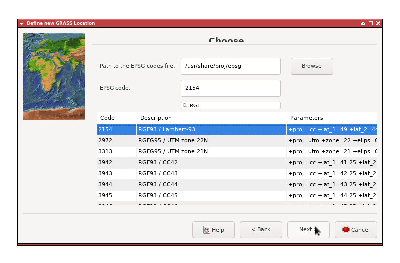
\includegraphics[width=0.70\hsize]{capture0.eps}
\caption{La procédure de création de localisation de GRASS GIS invite l'utilisateur à préciser un système de coordonnées de référence.}
\label{fig:location}
\end{center}
\end{figure}

Cette étape peut aussi être effectuée à la console avec la commande suivante :

\begin{code}
grass79 -c EPSG:2154 L93
\end{code}

GRASS GIS permet de gérer des données matricielles (raster), des données vectorielles (vector), des données attributaires. Le module \verb+r.avac+ fait appel à ces trois types de données.

\subsection{Données raster : importation de données topographiques}
Le fichier \texttt{boussolenc.gpkg} est un geopackage dont les données sont référencées dans le système Lambert 93. Il comporte un modèle numérique de terrain nommé \texttt{topo}, et une carte de relief ombré nommée \texttt{ombrage} que l'on va importer dans notre localisation en passant les commandes suivantes au terminal :

\begin{code}
r.in.gdal input=boussolenc.gpkg gdal\_doo='table=topo\_2m' output=topo

r.in.gdal input=boussolenc.gpkg gdal\_doo='table=ombrage' output=ombrage
\end{code}

Dans la fenêtre \emph{Layer Manager} l'utilisateur peut ajouter ces cartes à la vue (voir figure \ref{fig:shade}).

\begin{figure}[!h]
\begin{center}
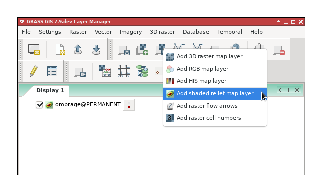
\includegraphics[width=0.70\hsize]{capture3.eps}
\caption{Le menu \emph{Add various raster map layers > Add shaded relief map} permet de combiner le relief ombré et le fichier topo.}
\label{fig:shade}
\end{center}
\end{figure}

Pour alimenter AVAC, \verb+r.avac+ transforme cette carte raster, qu'elle adressera au code sous la forme d'un fichier nommé \texttt{topo.asc}. La résolution et l'extension géographique du fichier sont contrôlées par l'utilisateur lors de la définition de la région de travail.


\subsection{Notion de région}

Une notion centrale de GRASS GIS est ce qu'on appelle la \emph{région}. Il s'agit d'un ensemble de valeurs numériques indiquant au programme la position, l'étendue, et la résolution d'une grille qui discrétise la zone de travail. Par défaut dans une localisation vierge, cette région est définie par une seule cellule située à l'origine du repère cartésien de la projection courante. \comment{\dbend}\textbf{Si l'on veut que GRASS traite nos données correctement il importe avant tout d'indiquer les paramètres de région correspondant à notre zone de travail}. Dans le cas présent il suffit de lancer la commande suivante pour faire coïncider la région avec l'extension et la résolution du modèle numérique de terrain importé à l'étape précédente :

\begin{code}
g.region -p rast=topo
\end{code}

L'argument \texttt{-p} force l'affichage des nouveaux paramètres de région en sortie.

La fenêtre d'affichage des cartes permet de visualiser la région courante (voir figure \ref{fig:raster}). On peut aussi définir soi-même l'extension de la région de façon interactive dans la fenêtre d'affichage des cartes (icône Various zoom options > set computational region extent interactively).

Enfin est possible, et souhaitable, de fixer la résolution à laquelle nous souhaitons travailler. La commande précédente nous apprend que le pas d'échantillonnage de la topographie que nous avons importée est de 2\,m ; on peut décider de vouloir travailler à un pas de 5\,m, en donnant l'instruction suivante :

\begin{code}
g.region -pa res=5
\end{code}

L'argument \texttt{-a} force la définition d'une région dont les dimensions sont des multiples de la résolution demandée.

\begin{figure}[!h]
\begin{center}
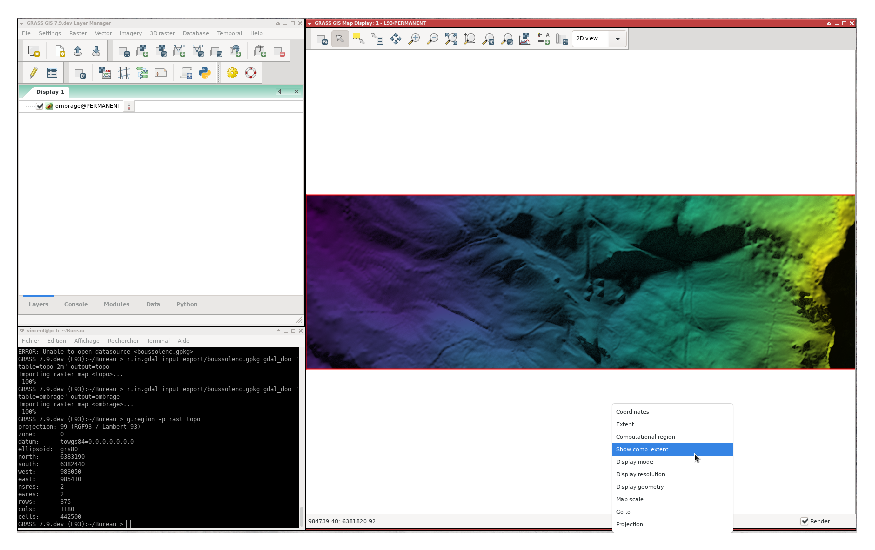
\includegraphics[width=1\hsize, angle=00]{capture1.eps}
\caption{affichage en relief ombré du modèle numérique de terrain. La fenêtre \emph{map display} permet d'afficher la région courante sous la forme d'un cadre rouge.}
\label{fig:raster}
\end{center}
\end{figure}

La version actuelle de \verb+r.avac+ gère de façon rudimentaire la fonctionnalité AMR (adaptive mesh refinement) ; pour indiquer à Geoclaw de travailler à un niveau de grille supérieur sur une portion de la zone de calcul, on peut préciser au module (option amr) une zone rectangulaire qu'on aura préalablement déterminée dans GRASS au moyen d'une carte vecteur comportant un polygone dont l'identifiant \texttt{cat} porte la valeur du facteur amr souhaité (actuellement le code ne prend en charge que le niveau 2). Une manière commode de procéder est la suivante :
\bei
\item définir comme précédemment l'extension d'une région de façon interactive dans la fenêtre d'affichage des cartes ;
\item créer une carte vectorielle comportant un rectangle aux dimensions de la région ainsi définie, avec la commande 

\begin{code}
v.in.region cat=2 out=amr2 --o
\end{code}
\eit

\subsection{Données vecteur : importation et création de données vectorielles}

Le fichier \texttt{boussolenc.gpkg} comporte une couche vectorielle de courbes de niveau qui peut être importée comme suit :

\begin{code}
v.in.ogr in=boussolenc.gpkg layer='cbn' out=cbn
\end{code}

Superposée à l'affichage des cartes raster précédentes, elle offre une meilleure visibilité du relief de notre jeu de données exemple.

Le code AVAC a besoin de connaître la localisation des zones de départ des avalanches, ainsi que la hauteur de neige mobilisée pour chacune. Le module \verb+r.avac+ récupère cette donnée initiale sous la forme d'une carte vecteur que nous nommerons \texttt{ZA}, comportant autant de polygones qu'il y a de zones de départ ; la hauteur de neige dans chacun des panneaux est portée par un attribut que nous nommons \texttt{h}.

Le fichier \texttt{boussolenc.gpkg} comporte un exemple de couche vectorielle nommé \texttt{ZA} répondant au format attendu par \verb+r.avac+. Pour l'importer dans GRASS, exécuter la commande suivante :

\begin{code}
v.in.ogr in=boussolenc.gpkg layer='ZA' out=ZA
\end{code}

Les commandes suivantes permettent de s'assurer que le champ \texttt{h} est bien présent dans la table attributaire de la couche ZA :

\begin{code}
v.db.connect ZA -p

db.columns ZA
\end{code}

L'utilisateur se reportera à la documentation de GRASS GIS pour une présentation du modèle vectoriel\footnote{\href{https://grass.osgeo.org/grass76/manuals/vectorintro.html}{https://grass.osgeo.org/grass76/manuals/vectorintro.html}} et attributaire\footnote{\href{https://grasswiki.osgeo.org/wiki/Vector\_Database\_Management}{https://grasswiki.osgeo.org/wiki/Vector\_Database\_Management}},  et l'utilisation des outils d'édition \footnote{\href{https://grass.osgeo.org/grass76/manuals/wxGUI.vdigit.html}{https://grass.osgeo.org/grass76/manuals/wxGUI.vdigit.html}}. (voir figure \ref{fig:vector})


\begin{figure}[!h]
\begin{center}
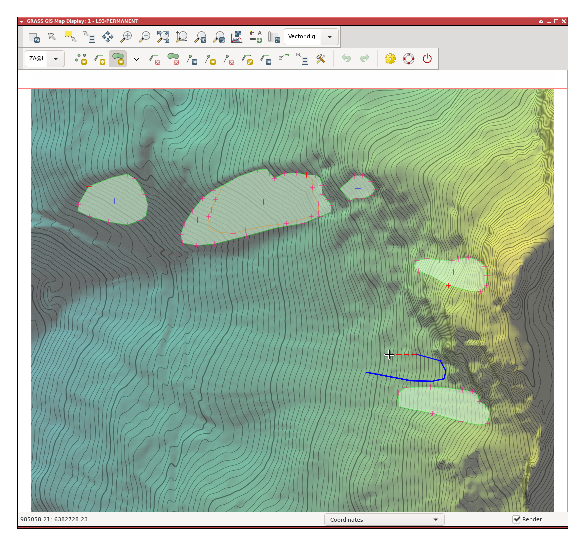
\includegraphics[width=0.70\hsize]{capture2.eps}
\caption{La couche vectorielle ZA peut être éditée pour modifier, ajouter, supprimer des zones de départ.}
\label{fig:vector}
\end{center}
\end{figure}

Pour alimenter AVAC, \verb+r.avac+ discrétise cette carte vectorielle, qu'elle adressera au code sous la forme d'un fichier nommé \texttt{initials.xyz}.


\subsection{Fonctionnalités de \texttt{r.avac}}

\paragraph{Loi rhéologique}
Le code AVAC offre le choix entre deux lois de comportement de la neige. 
L'expression des frottements peut suivre :
\bei
\item une loi de \emph{Voellmy} (à deux paramètres $\mu$, $\xi$), ou
\item une loi de \emph{Coulomb} (à un paramètre $\mu$).
\eit
L'argument \texttt{rheology} de \verb+r.avac+ permet de choisir l'une ou l'autre de ces lois : 
\bei
\item \texttt{rheology=0} pour Voellmy, choix par défaut ;
\item \texttt{rheology=1} pour Coulomb.
\eit
Le choix rheology=1 rend inopérant le paramètre $\xi$.

\paragraph{Hauteurs de neige}
Dans sa dernière version \verb+r.avac+ procède à une modulation de la hauteur de neige fournie par le paramètre \texttt{depth} ou l'attribut \texttt{h}, en fonction de la raideur de la pente en chaque point de la zone de départ. Le module utilise une variation de la formule de Quervain :
\[
h(z) = h_0(z) \frac{\sin\theta_{ref}-\nu \cos\theta_{ref}}{\sin\theta -\nu \cos\theta},
\]

où $h_0$ est le cumul de neige à plat à une altitude $z$ donnée, $\theta_{ref}$ est un angle de référence (pente pour laquelle le facteur de correction serait 1),   $\theta$ l'angle de pente du panneau à l'altitude $z$, et $\nu$ un coefficient empirique. Les valeurs par défaut $\nu=0,2$ et $\theta_{ref}=30$\degres{} peuvent être modulées directement dans le code source de \verb+r.avac+.


Cette version de \verb+r.avac+ permet également de définir plus finement la hauteur de neige dans la zone de départ : il est possible d'indiquer un gradient hypsométrique de hauteur de neige grâce à l'argument \texttt{grad}, qui se décline sous la forme d'un triplet (hauteur,gradient,altitude). Par exemple

\begin{code}
\texttt{grad=1.8,0.03,1850} 
\end{code}

signifie que la hauteur de neige vaut 180\,cm à 1850\,m d'altitude, et le gradient hypsométrique est de 3\,cm par tranche de 100\,m de dénivellation. Lorsque cette option est donnée à \verb+r.avac+, la valeur calculée pour chaque maille de la grille écrase la valeur fournie par l'attribut \texttt{h} de la carte \texttt{ZA}.



\section{Exécution}

\subsection{Syntaxe}
La commande \verb+r.avac+ peut être lancée depuis le terminal en mode textuel, mais pour se familiariser avec la commande il est commode d'appeler l'interface graphique du module. Pour cela taper simplement dans le terminal :

\begin{code}
r.avac --ui
\end{code}

Il suffit alors de renseigner correctement les arguments obligatoires figurant dans l'onglet \emph{Required}. L'onglet \emph{Optional} comporte des arguments dont les valeurs sont renseignées par défaut, notamment les paramètres de calage du modèle AVAC (voir documentation AVAC).

\clearpage
L'argument \texttt{--h} renvoie la syntaxe complète de la commande :

\begin{code}
r.avac --h
\begin{Verbatim}
Usage:
 r.avac [-mrc] simul=name dem=name za=name [depth=name] [amr=name]
   [dt=string] [t=string] [rheology=string] [rho=string] [xi=string]
   [mu=string] [grad=string] [vthres=string] [bslope=string]
   [--overwrite] [--help] [--verbose] [--quiet] [--ui]

Flags:
  -m   compute max(h) and max(p) maps throughout simul strds
  -r   reset existing simul strds
  -c   run geoclaw 'make clobber'

Parameters:
     simul   output simulation STRDS
       dem   input elevation raster map
        za   input starting area vector map
     depth   depth column for starting area
       amr   input AMR zone map
        dt   time increment
             default: 20
         t   simulation duration
             default: 100
  rheology   type of rheology
             default: 0
       rho   snow density
             default: 300
        xi   Voellmy xi
             default: 1500
        mu   Voellmy mu
             default: 0.15
      grad   depth hypsometric gradient
    vthres   velocity threshold
             default: 0.05
    bslope   beta slope
             default: 1.1
\end{Verbatim}
\end{code}

Avec un peu d'habitude, l'utilisateur lancera \verb+r.avac+ depuis la console GRASS. Par exemple :

\begin{code}
r.avac -mr simul=sim2 rheology=0 dem=topo za=ZA dt=1 t=40 \backslash 

mu=0.2 xi=800 rho=300 grad=1.7,0.03,1850 amr=amr2 vthres=0.2
\end{code}

L'intérêt d'invoquer la ligne de commande plutôt que l'interface graphique est que l'on peut facilement faire plusieurs itérations du code en changeant un seul paramètre, et ce en profitant du rappel de l'historique des commandes au prompt GRASS.

\subsection{Fonctionnement}

Lorsque la commande est lancée, le script se charge d'alimenter le code AVAC avec les données topographiques (topo.asc), les conditions initiales (initials.xyz), l'extension géographique du calcul (conforme aux paramètres de région fixés précédemment), les paramètres du calcul (voellmy.data, AddSetrun.py, et setrun.py).

Le calcul effectué, \verb+r.avac+ traite les fichiers \texttt{fort.qxxxx} produits par AVAC afin d'importer dans GRASS les paramètres $h(t)$ et $p(t)=\frac{1}{2}\varrho {u}^2$, où  $\varrho$ et ${u}$ sont respectivement la densité de la neige et la vitesse. Suit un travail d'assemblage des multiples grilles générées par le code pour obtenir une série de rasters décrivant l'écoulement au pas de temps \texttt{dt} indiqué en entrée. En reprenant l'exemple de commande précédent, les rasters \texttt{h.sim2\_xxxx} et \texttt{p.sim2\_xxxx} sont incorporés dans deux séries temporelles (spatio-temporal raster dataset, strds), l'une nommée \texttt{sim2\_h} décrivant la hauteur d'écoulement (exprimée en m), l'autre nommée \texttt{sim2\_p} décrivant la pression au sein de l'écoulement (exprimée en kPa).

Si l'utilisateur souhaite interrompre l'exécution du code, il peut le faire en mode graphique en appuyant sur le bouton Stop ; en mode console c'est le raccourci  $<$ctrl+c$>$ qui envoie le signal d'interruption. Le script effectue des opérations de nettoyage avant de quitter (purge de certains paramètres, suppression de fichiers temporaires).

\section{Visualiser, exporter}

L'utilisateur peut visualiser le résultat de la simulation en lançant le module interactif \texttt{g.gui.animation}.

On peut aisément modifier la charte colorimétrique associée à chaque série. Par exemple si on souhaite appliquer la charte des pressions utilisée dans les documents Toraval, qui est consignée dans le fichier \texttt{p\_toraval.file} joint à notre archive :

\begin{code}
t.rast.colors input=sim5\_h rules=[/path\_to/]p\_toraval.file
\end{code}


Le module \texttt{g.gui.animation} propose l'export d'animations sous plusieurs formes. Lorsque le nombre de cartes de la série est grand (typiquement un millier d'itérations), il n'est plus possible de visualiser ni d'exporter la série. L'utilisa\-teur peut alors choisir d'exporter une série d'images au format png en vue d'un post-traitement avec d'autres outils, comme par exemple l'utilitaire \verb+ffmpeg+ :

\begin{code}
\begin{Verbatim}
g.list rast | grep h.sim2 | parallel r.out.png in={} out={}
ffmpeg -f image2 -r 12 -i "h.sim2_0\%03d.png" -vcodec png out_h.avi

g.list rast | grep p.sim2 | parallel r.out.png in={} out={}
ffmpeg -f image2 -r 12 -i "p.sim2_0\%03d.png" -vcodec png out_p.avi
\end{Verbatim}
\end{code}


\newpage

~\vfill

\begin{figure}[!h]
\begin{center}
\includegraphics[width=0.70\hsize]{capture4.eps}
\caption{Exemple de post-traitement réalisé avec Blender pour produire une animation combinant hauteur d'écoulement (déplacement) et pression (couleur). Voir la vidéo à l'adresse \href{http://telec.toraval.fr/boussolenc.avi}{http://telec.toraval.fr/boussolenc.avi}}.
\label{fig:blend}
\end{center}
\end{figure}

~\vfill

\end{document}
